% VUT FIT MITAI
% MSZ 2021/2022
% Author: Vladimir Dusek
% Login: xdusek27

%%%%%%%%%%%%%%%%%%%%%%%%%%%%%%%%%%%%%%%%%%%%%%%%%%%%%%%%%%%%%%%%%%%%%%%%%%%%%%%%

% Path to figures
\graphicspath{{msp/markovske_retezce/figures}}

%%%%%%%%%%%%%%%%%%%%%%%%%%%%%%%%%%%%%%%%%%%%%%%%%%%%%%%%%%%%%%%%%%%%%%%%%%%%%%%%

\chapter{MSP~--~Markovské řetězce a základní techniky pro jejich analýzu.}

%%%%%%%%%%%%%%%%%%%%%%%%%%%%%%%%%%%%%%%%%%%%%%%%%%%%%%%%%%%%%%%%%%%%%%%%%%%%%%%%

\section{Zdroje}

\begin{compactitem}
    \item \path{MSP_11_Markov_chains.pdf}
    \item \path{MSP_12_Markov_decision_processes.pdf}
    \item \path{MSP_2021-11-30_1080p.mp4}
    \item \path{MSP_2021-12-07_1080p.mp4}
\end{compactitem}

%%%%%%%%%%%%%%%%%%%%%%%%%%%%%%%%%%%%%%%%%%%%%%%%%%%%%%%%%%%%%%%%%%%%%%%%%%%%%%%%

\section{Úvod a kontext}

\begin{compactitem}
    \item Markovské řetězce a další pravděpodobnostní modely slouží pro modelování náhodných (stochastických) systémů.

    \item Stochastické systémy můžeme dělit podle: \begin{compactitem}
        \item času (spojitý / diskrétní),
        \item způsobu rozhodování (plně pravděpodobnostní /  nedeterministické),
        \item velikosti stavového prostoru (konečný / nekonečný),
        \item pozorovatelnosti prostředí (plně pozorovatelné prostředí / částečně pozorovatelné prostředí).
    \end{compactitem}
\end{compactitem}

\begin{figure}[H]
    \centering
    \includegraphics[width=1\linewidth]{branches.pdf}
    \caption{Deterministické, nedeterministické a pravděpodobnostní větvení.}
\end{figure}

\begin{figure}[H]
    \centering
    \includegraphics[width=0.6\linewidth]{modelovani_pravdepodobnostnich_systemu.pdf}
    \caption{Dělení pravděpodobnostních modelů na základě času a způsobu rozhodování.}
\end{figure}

%%%%%%%%%%%%%%%%%%%%%%%%%%%%%%%%%%%%%%%%%%%%%%%%%%%%%%%%%%%%%%%%%%%%%%%%%%%%%%%%

\section{Markovské řetězce}

\begin{compactitem}
    \item Markovské řetězce (DTMC, \textit{Discrete-Time Markov Chains}) jsou pravděpodobnostní modely, které májí: \begin{compactitem}
        \item diskrétní čas,
        \item plně pravděpodobnostní způsob rozhodování,
        \item konečný stavový prostor,
        \item plně pozorovatelné prostředí.
    \end{compactitem}

    \item Formálně, markovský řetězec je čtveřice $D = (S, s_0, P, L)$, kde \begin{compactitem}
        \item $S$ je konečná množina stavů;
        \item $s_0 \in S$ je výchozí stav (může být zobecněn jako výchozí pravděpodobnostní distribuce);
        \item $P : S \times S \rightarrow \langle 0, 1 \rangle$ je pravděpodobnostní přechodová matice, pro kterou platí: $$ \forall s \in S \sum_{s' \in S} P(s, s') = 1 $$
        \item $L : S \rightarrow 2^{AP}$ je funkce označující stavy.
    \end{compactitem}

    \item Pravděpodobnost přechodu závisí pouze na aktuálním stavu (\textit{memorylessness}).

\end{compactitem}

\paragraph*{Cesta} Cesta je posloupnost stavů $\langle s_0, s_1, s_2, \dots \rangle$ pro kterou platí $\forall i ~ P(s_i, s_{i+1}) > 0$.

\paragraph*{Pravděpodobnost cesty} Pravděpodobnost ($Pr$, \textit{probability measure}) konečné cesty $\omega = \langle s_0, s_1, s_2, \dots, s_n \rangle$ je: \begin{compactitem}
    \item $Pr(s_0) = 1$
    \item $Pr( s_0, s_1, s_2, \dots, s_n ) = P(s_0, s_1) \cdot P(s_1, s_2) \cdot \ldots \cdot P(s_{n-1}, s_n) $.
\end{compactitem}

\paragraph*{Příklad 1} Pravděpodobnostní systém doručování zpráv. Význam stavů: \begin{compactitem}
    \item start -- $s_0$;
    \item zpráva byla doručena -- $s_3$;
    \item zpráva byla ztracena -- $s_2$;
    \item odesílání -- $s_1$.
\end{compactitem}

\begin{figure}[H]
    \centering
    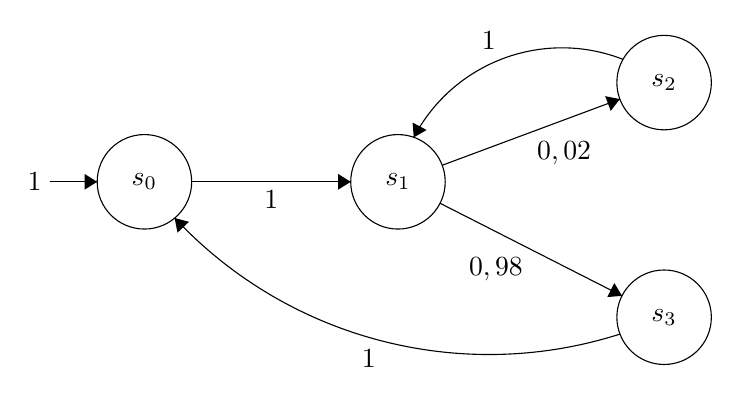
\begin{tikzpicture}[scale=0.2]
        \tikzstyle{every node}+=[inner sep=0pt]
        \draw [black] (20.6,-21) circle (3);
        \draw (20.6,-21) node {$s_0$};
        \draw [black] (36.7,-21) circle (3);
        \draw (36.7,-21) node {$s_1$};
        \draw [black] (53.6,-14.7) circle (3);
        \draw (53.6,-14.7) node {$s_2$};
        \draw [black] (53.6,-29.6) circle (3);
        \draw (53.6,-29.6) node {$s_3$};
        \draw [black] (23.6,-21) -- (33.7,-21);
        \fill [black] (33.7,-21) -- (32.9,-20.5) -- (32.9,-21.5);
        \draw (28.65,-21.5) node [below] {$1$};
        \draw [black] (14.6,-21) -- (17.6,-21);
        \draw (14.1,-21) node [left] {$1$};
        \fill [black] (17.6,-21) -- (16.8,-20.5) -- (16.8,-21.5);
        \draw [black] (39.51,-19.95) -- (50.79,-15.75);
        \fill [black] (50.79,-15.75) -- (49.86,-15.56) -- (50.21,-16.5);
        \draw (47.25,-18.4) node [below] {$0,02$};
        \draw [black] (39.37,-22.36) -- (50.93,-28.24);
        \fill [black] (50.93,-28.24) -- (50.44,-27.43) -- (49.99,-28.32);
        \draw (42.92,-25.81) node [below] {$0,98$};
        \draw [black] (50.799,-30.669) arc (-72.26281:-136.95066:27.308);
        \fill [black] (22.52,-23.3) -- (22.7,-24.23) -- (23.43,-23.54);
        \draw (34.84,-31.65) node [below] {$1$};
        \draw [black] (37.703,-18.183) arc (152.308:68.581:10.63);
        \fill [black] (37.7,-18.18) -- (38.52,-17.71) -- (37.63,-17.24);
        \draw (42.47,-12.64) node [above] {$1$};
    \end{tikzpicture}
    \caption{Pravděpodobnostní systém doručování zpráv modelpván pomocí markovského řetězce.}
\end{figure}

\begin{compactitem}
    \item Jaká je pravděpodobnost, že zpráva byla úspěšně přijata do 5ti kroků?
    $$ Pr(s_0, s_1, s_3) + Pr(s_0, s_1, s_2, s_1, s_3) = 0,98 + 0,02 + 0,098 = 0,9996 $$

    \item Jaká je pravděpodobnost, že zpráva bude někdy doručena?
    $$ \sum_{n=0}^{\infty} Pr(s_0, (s_1, s_2)^n, s_3) = \sum_{n=0}^{\infty} 0,02^n \cdot 0,98 = 1 $$
\end{compactitem}

\paragraph*{Příklad 2} Pravděpodobnostní systém pro namodelování férové mince pomocí \uv{cinklé} mince (nevíme jak).

\begin{figure}[H]
    \centering
    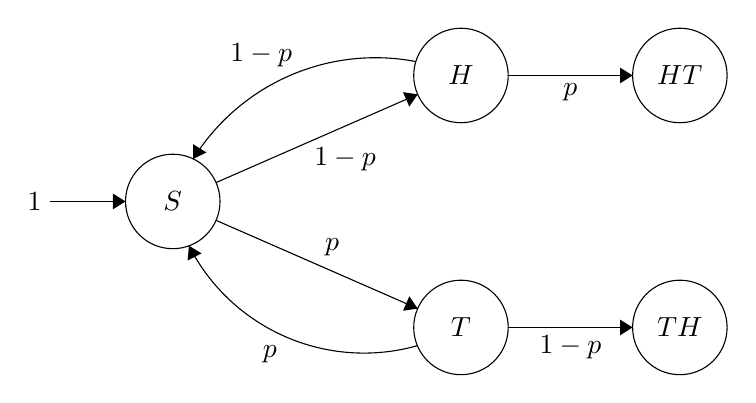
\begin{tikzpicture}[scale=0.2]
        \tikzstyle{every node}+=[inner sep=0pt]
        \draw [black] (24.3,-25.3) circle (3);
        \draw (24.3,-25.3) node {$S$};
        \draw [black] (42.6,-17.3) circle (3);
        \draw (42.6,-17.3) node {$H$};
        \draw [black] (42.6,-33.3) circle (3);
        \draw (42.6,-33.3) node {$T$};
        \draw [black] (56.5,-33.3) circle (3);
        \draw (56.5,-33.3) node {$TH$};
        \draw [black] (56.5,-17.3) circle (3);
        \draw (56.5,-17.3) node {$HT$};
        \draw [black] (16.5,-25.3) -- (21.3,-25.3);
        \draw (16,-25.3) node [left] {$1$};
        \fill [black] (21.3,-25.3) -- (20.5,-24.8) -- (20.5,-25.8);
        \draw [black] (27.05,-26.5) -- (39.85,-32.1);
        \fill [black] (39.85,-32.1) -- (39.32,-31.32) -- (38.92,-32.24);
        \draw (34.42,-28.79) node [above] {$p$};
        \draw [black] (27.05,-24.1) -- (39.85,-18.5);
        \fill [black] (39.85,-18.5) -- (38.92,-18.36) -- (39.32,-19.28);
        \draw (35.24,-21.82) node [below] {$1-p$};
        \draw [black] (25.595,-22.6) arc (148.08025:79.14565:13.639);
        \fill [black] (25.59,-22.6) -- (26.44,-22.19) -- (25.59,-21.66);
        \draw (29.92,-16.79) node [above] {$1-p$};
        \draw [black] (39.839,-34.456) arc (-74.1755:-153.05041:12.467);
        \fill [black] (25.33,-28.11) -- (25.24,-29.05) -- (26.13,-28.6);
        \draw (30.47,-34.4) node [below] {$p$};
        \draw [black] (45.6,-17.3) -- (53.5,-17.3);
        \fill [black] (53.5,-17.3) -- (52.7,-16.8) -- (52.7,-17.8);
        \draw (49.55,-17.8) node [below] {$p$};
        \draw [black] (45.6,-33.3) -- (53.5,-33.3);
        \fill [black] (53.5,-33.3) -- (52.7,-32.8) -- (52.7,-33.8);
        \draw (49.55,-33.8) node [below] {$1-p$};
    \end{tikzpicture}
    \caption{Pravděpodobnostní systém pro namodelování férové mince pomocí \uv{cinklé} mince.}
\end{figure}

%%%%%%%%%%%%%%%%%%%%%%%%%%%%%%%%%%%%%%%%%%%%%%%%%%%%%%%%%%%%%%%%%%%%%%%%%%%%%%%%

\section{Analýza přechodů (\textit{transient analysis})}

\begin{compactitem}
    \item Vysvětlení: \begin{compactitem}
        \item $t_k(s)$ vyjadřuje pravděpodobnost, že po spuštění procesu z počátečního stavu $s_0$, se nacházím ve stavu $s \in S$ v čase $k \geq 0$.
    \end{compactitem}

    \item Formálně:
    $$ t_k(s) = P[X(k) = s ~|~ X(0) = s_0] $$

    \item Můžeme použít pravděpodobnost $Pr$ a vypsat všechny cesty délky $k$, které vedou do $s$ -- exponenciální složitost $\mathcal{O}(e^k)$.

    \item Nebo lépe, můžeme využít vlastnost \textit{memorylessness} a dostat se na lineární složitost $\mathcal{O}(k)$ (pravděpodobnost přechodu v čase $k-1$ z nějakého předchůdce $s$ do $s$).
    $$ t_0(s_0) = 1 ~,~ t_0(s) = 0 ~,~ s \not= s_0 $$
    $$ t_k(s) = \sum_{s' \in S} t_{k-1}(s') \cdot P(s', s) $$
\end{compactitem}

\paragraph*{Příklad 3} Modelování protokolu házení férovou šestistrannou kostkou pomocí férové mince (\textit{Knuth-Yao dice}).

\begin{figure}[H]
    \centering
    \includegraphics[width=0.75\linewidth]{priklad_2.pdf}
    \caption{Modelování protokolu házení férovou šestistrannou kostkou pomocí férové mince. Stavy reprezentující výsledek hodu kostkou mají \textit{self-loop} s pravděpodobnostní $1$ a značme je $r_i$ pro $i \in \{ 1, 2, \dots, 6 \}$.}
\end{figure}

\begin{compactitem}
    \item Tranzientní analýza ze stavu $s_1$: \begin{compactitem}
        \item pro $k = 1 ~:~ s_2 = s_5 = 0,5$
        \item pro $k = 2 ~:~ s_3 = s_4 = s_6 = s_7 = 0,25$
        \item pro $k = 3 ~:~ s_2 = s_5 = r_1 = r_2 = \ldots = r_6 = 0,125 $
        \item pro $k = 5 ~:~ i \in \{ 1, 2, \dots, 6 \} ~:~ r_i = (0,5)^3 + (0,5)^5 = 0,156$
    \end{compactitem}
\end{compactitem}

%%%%%%%%%%%%%%%%%%%%%%%%%%%%%%%%%%%%%%%%%%%%%%%%%%%%%%%%%%%%%%%%%%%%%%%%%%%%%%%%

\section{Analýza ustáleného stavu (\textit{steady state analysis})}

\begin{compactitem}
    \item Vysvětlení: \begin{compactitem}
        \item $t_{\infty}(s)$ vyjadřuje pravděpodobnost, že po spuštění procesu z počátečního stavu $s_0$, se nacházím ve stavu $s \in S$ v čase $k = \infty$.

        \item Přesněji:
        $$ t_{\infty}(s) = \lim_{k \rightarrow \infty}{t_k(s)} $$
    \end{compactitem}

    \item Zkoumání chování systému po uplynutí \uv{nekonečno} kroků.

    \item Jde o ustálené rozdělení pravděpodobnosti napříč stavy -- pokud bychom udělali ještě jeden krok navíc, tak už nezmění.

    % \item Pro tzv. periodické markovské řetězce limita pro $k \rightarrow \infty$ neexistuje.

\end{compactitem}

\subsection{Neredukovatelné markovské řetězce}

\begin{compactitem}
    \item Celý model je z hlediska teorie grafů silně souvislá komponenta -- Z každého stavu se lze dostat do každého dalšího stavu.

    \item Výsledné pravděpodobnostní rozdělení nezávisí na počátečním stavu.

    \item Lze spočítat pomocí tzv. balančních rovnic:
    $$ \forall s \in S : t_{\infty}(s) = \sum_{s' \in S} t_{\infty}(s') \cdot P(s', s) $$
    $$ \sum_{s \in S} t_{\infty}(s) = 1$$

\end{compactitem}

\paragraph*{Příklad 4} Uvažme následující model.

\begin{figure}[H]
    \centering
    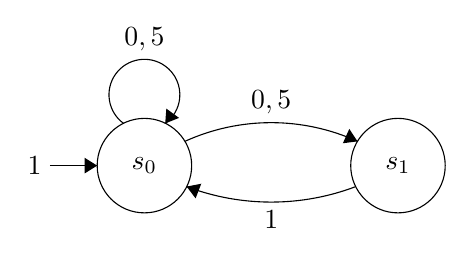
\begin{tikzpicture}[scale=0.2]
        \tikzstyle{every node}+=[inner sep=0pt]
        \draw [black] (20.6,-21) circle (3);
        \draw (20.6,-21) node {$s_0$};
        \draw [black] (36.7,-21) circle (3);
        \draw (36.7,-21) node {$s_1$};
        \draw [black] (23.167,-19.46) arc (114.46612:65.53388:13.239);
        \fill [black] (34.13,-19.46) -- (33.61,-18.67) -- (33.2,-19.58);
        \draw (28.65,-17.77) node [above] {$0,5$};
        \draw [black] (14.6,-21) -- (17.6,-21);
        \draw (14.1,-21) node [left] {$1$};
        \fill [black] (17.6,-21) -- (16.8,-20.5) -- (16.8,-21.5);
        \draw [black] (19.277,-18.32) arc (234:-54:2.25);
        \draw (20.6,-13.75) node [above] {$0,5$};
        \fill [black] (21.92,-18.32) -- (22.8,-17.97) -- (21.99,-17.38);
        \draw [black] (34.018,-22.333) arc (-69.24413:-110.75587:15.147);
        \fill [black] (23.28,-22.33) -- (23.85,-23.08) -- (24.21,-22.15);
        \draw (28.65,-23.82) node [below] {$1$};
    \end{tikzpicture}
    \caption{Markovův řetězec.}
\end{figure}

\begin{compactitem}
    \item Sestavíme následující soustavu rovnic:
    $$ x_0 = 0,5x_0 + x_1 $$
    $$ x_1 = 0,5x_0 $$

    \item Řešení:
    $$ x_0 = \frac{2}{3} ~;~ x_1 = \frac{1}{3}$$
\end{compactitem}

\subsection{Obecné (aperiodické) markovské řetězce} \begin{compactitem}

    \item Model je tvořen několika souvislýma komponentama (SCC). \begin{compactitem}
        \item Dále rozlišujeme ještě tzv. \textit{bottom} silně souvislé komponenty (BSCC), to jsou takové, ze kterých už se není možné dostat.
    \end{compactitem}

    \item Výsledné pravděpodobnostní rozdělení závisí na počátečním stavu.
\end{compactitem}

\begin{figure}[H]
    \centering
    \includegraphics[width=0.6\linewidth]{ss-general.pdf}
    \caption{Příklad markovského řetězce, který je tvořem 4 silně souvislýma komponentama, z čehož 3 jsou \textit{bottom} silně souvislé.}
\end{figure}

\begin{compactitem}
    \item Stavy dělíme na: \begin{compactitem}
        \item Přechodové stavy -- stavy mimo BSCC ($s_t$):
        $$ t_{\infty} (s_t) = 0 $$
        \item Rekurentní stavy -- stavy uvnitř BSCC ($s_r$):
        $$ t_{\infty} (s_r) > 0 $$
    \end{compactitem}

    \item Výpočet: Součin pravděpodobnosti, že se dostanu do dané BSCC a pravděpodobnostni, že se dostanu do daného stavu uvnitř BSCC.

\end{compactitem}

%%%%%%%%%%%%%%%%%%%%%%%%%%%%%%%%%%%%%%%%%%%%%%%%%%%%%%%%%%%%%%%%%%%%%%%%%%%%%%%%

\section{Problém dosažitelnosti stavu (\textit{reachability problem})}

\begin{compactitem}
    \item Nechť $T \subseteq S$ je nějaká cílová množina.

    % \item Cíl: pro každý stav spočítat pravděpodobnost, že když v něm začnu, tak s jakou pravděpodobností se dostanu do nějakého stavu $s \in T$.

    \item Vysvětlení: \begin{compactitem}
        \item $x(s)$ vyjadřuje pravděpodobnost, že se dostanu do stavu $s' \in T$, pokud začínám ve stavu $s \in S$.
    \end{compactitem}

    \item Proč to dělat? Zjistím s jakou pravděpodobností se dostanu do cílových stavů (viz další příklad).

    \item Postup: \begin{compactenum}
        \item Všechny cílové stavy nastavíme jako tzv. absorbující (pokud ho dosáhneme, tak už ho neopustíme).
        $$ \forall s \in T : P(s, s) = 1 $$

        \item Spočítáme množinu stavů $S_{no} \subset S$, která obsahuje stavy, ze kterých nevede žádná cesta do nějakého stavu z množiny $T$.

        \item Vyřešíme soustavu rovnic:
        $$ x(s) = 1 ~,~ \forall s \in T $$
        $$ x(s) = 0 ~,~ \forall s \in S_{no} $$
        $$ x(s) = \sum_{s' \in S} P(s, s') \cdot x(s') ~,~ \forall s \not\in (T \cup S_{no}) $$

    \end{compactenum}
\end{compactitem}

\paragraph*{Příklad 5} Problém dosažitelnosti stavu pro protokol \uv{Modelování protokolu házení férovou šestistrannou kostkou pomocí férové mince}.

\begin{figure}[H]
    \centering
    \includegraphics[width=1\linewidth]{priklad_4.pdf}
    \caption{Příklad na problém dosažitelnosti. $T = \{ r_1, r_2, \ldots, r_6 \}$.}
\end{figure}

%%%%%%%%%%%%%%%%%%%%%%%%%%%%%%%%%%%%%%%%%%%%%%%%%%%%%%%%%%%%%%%%%%%%%%%%%%%%%%%%

\section{Očekávaný počet kroků (\textit{expected time to reach a state})}

\begin{compactitem}
    \item Nechť $T \subseteq S$ je nějaká cílová množina.

    \item Vysvětlení: \begin{compactitem}
        \item $e(s)$ vyjadřuje očekávaný (průměrný) počet kroků, že se dostanu do stavu $s' \in T$, pokud začínám ve stavu $s \in S$.
        \item Podmínka: pravděpodobnost dosáhnutí $s' \in T$ z $s$ musí být $1$.
    \end{compactitem}

    \item Postup: \begin{compactitem}
        \item Všechny cílové stavy nastavíme jako tzv. absorbující (pokud ho dosáhneme, tak už ho neopustíme).
        $$ \forall s \in T : P(s, s) = 1 $$

        \item Vyřešíme soustavu rovnic:
        $$ e(s) = 0 ~,~ \forall s \in T $$
        $$ e(s) = 1 + \sum_{s' \in S} P(s, s') \cdot e(s') ~,~ \forall s \not\in T $$
    \end{compactitem}

\end{compactitem}

\paragraph*{Příklad 6} Problém očekávaného počtu kroků pro protokol \uv{Modelování protokolu házení férovou šestistrannou kostkou pomocí férové mince}.

\begin{figure}[H]
    \centering
    \includegraphics[width=1\linewidth]{priklad_5.pdf}
    \caption{Příklad na očekávaný počet kroků. $T = \{ r_1, r_2, \ldots, r_6 \}$.}
\end{figure}
